\section{LEMAITRE: Hubble diagram project overview}

The LEMAITRE project aims at constructing the largest Hubble diagram by using an independent set of supernovae. One its objectives is to tackle the $(w_0-w_a)$ tension observed 
by recent results from \cite{Brout_2022}, \cite{Rubin_2023} and \cite{DES_2024} supernova analyses as well as the combination with BAO results from \cite{DESI_DR2_2025}. It is 
important to note that the low redshift supernova sample used in all three analyses is the same and that it seems to be the main motivating factor for the tension. 
By analyzing a completely new dataset for LEMAITRE, an independent assessment of this tension will be provided. Additionally with the LEMAITRE project comes a new 
analysis pipeline from end-to-end, starting from the lightcurve extraction and calibration up to the cosmological analysis. My work during the PhD involved the continued 
development and testing of a portion of the LEMAITRE pipeline named NaCl (see Chapter 3 and 4) which aims at training a spectrophotometric model. \\

\section{Datasets: ZTF, SNLS, HSC}

There are three datasets used in the LEMAITRE project: \\

\subsection{ZTF survey} \label{sec:ztf}
In this section we present the Zwicky Transient Facility survey as well as the the supernova sample that was primarily studied in this PhD the ZTF DR2. The ZTF camera is mounted on the Samuel Oschin 
48-inch (1.2m) telescope in the Mount Palomar Obsrevatory, California, USA. The primary purpose of the survey is the study of nearby astrophysical transients, which makes it 
really good for studying supernovae in the local Universe. \\

\begin{figure}[ht]
    \centering
    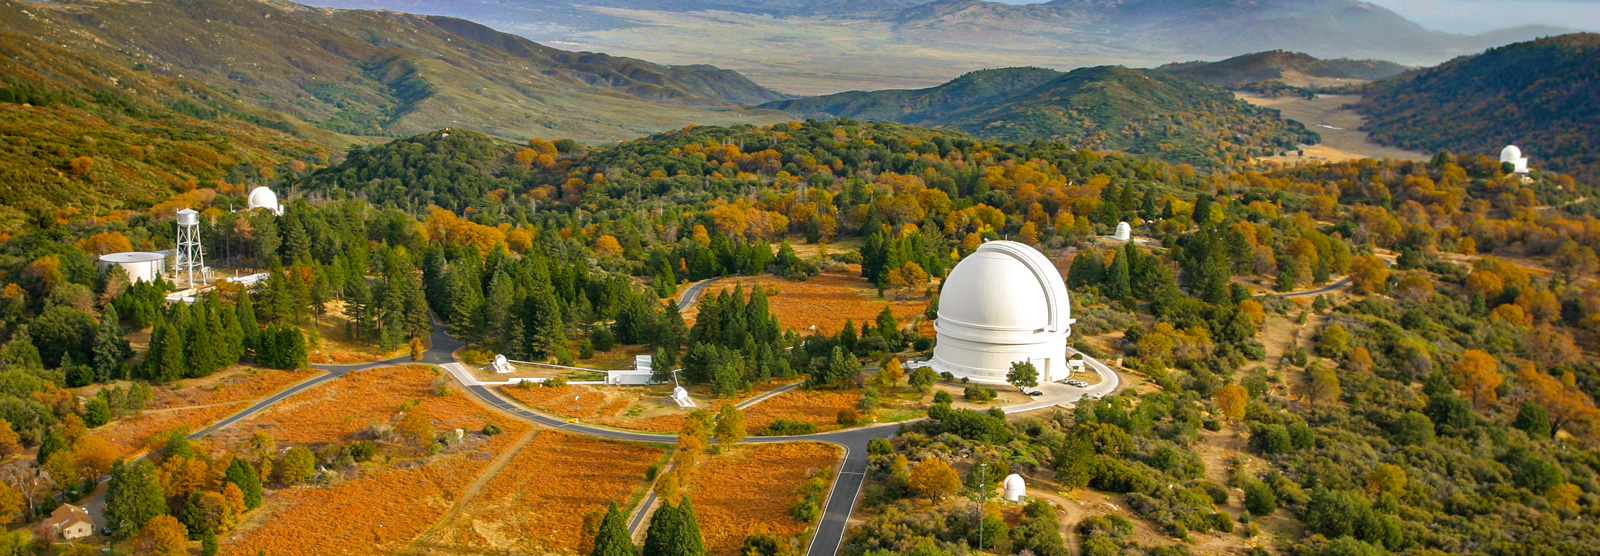
\includegraphics[width=1.0\textwidth]{MainLayout/Third_chapter/figures/palomar-observatory.jpg}
    \caption{Mount Palomar Observatory. Credits: Caltech \url{https://www.ztf.caltech.edu/} }
    \label{fig:palomar}
\end{figure}

\subsubsection{ZTF photometry}

The ZTF camera is made up of 16 CCDs (model e2v CCD231-C6) each possessing 6144 $\times$ 6160 pixels. The Samuel Oschin telescope contains a 1.2m mirror (called the "primary mirror" M1) that redirects the 
photons to the focal plane of the camera. The mirror is a spherical pyrex-glass mirror coated with aluminium which allows for a large observation field of view. 
The telescope also contains an aspherical lens at the entrance to correct for geometric aberrations. 
It covers a solid angle of $\sim 47 \text{deg}^2$ of the extragalactical northern sky and manages to conduct a full sky coverage twice per night. Each image covers approximately 235 times the area of the full moon. 
The photometry is done using 3 filters $g$, $r$ and $i$ covering the ranges of $\approx 4000 - 5500 \AA$, $\approx 5500 - 7000 \AA$ and $\approx 7000 - 9000 \AA$ respectively. 
It is important to highlight that the transmissions of the filters are sensor-dependent and we display them by averaging over the sensor transmissions. 
The magnitude limits for each band are $m_g \sim 20.8-21.1$mag, $m_r \sim 20.6-20.9$mag, $m_i \sim 19.9-20.2$mag where the variations are laregly due to the phases of the moon. 
The full details on the ZTF photometry are in \cite{Dekany_2020}. \\

\begin{figure}[ht]
    \centering
    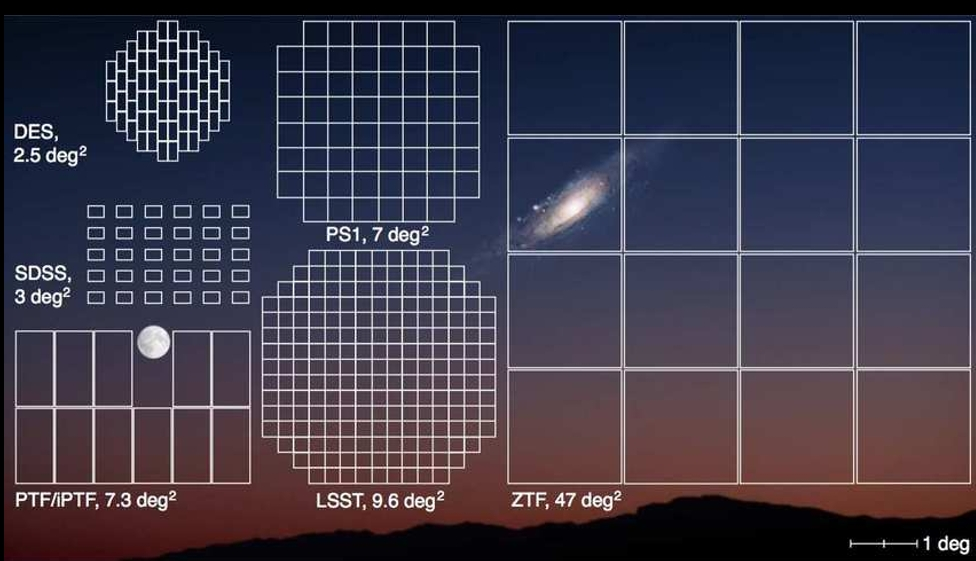
\includegraphics[width=0.8\textwidth]{MainLayout/Third_chapter/figures/ztf-camera-fov.jpg}
    \caption{Comparisons between the fields of view of ZTF, PS1, LSST, PTF, SDSS and DES. In the background we see in comparison the size of the moon and the Andromeda galaxy. Credits: Caltech \url{https://www.ztf.caltech.edu/} }
    \label{fig:ztf_fov}
\end{figure}

\begin{figure}[ht]
    \centering
    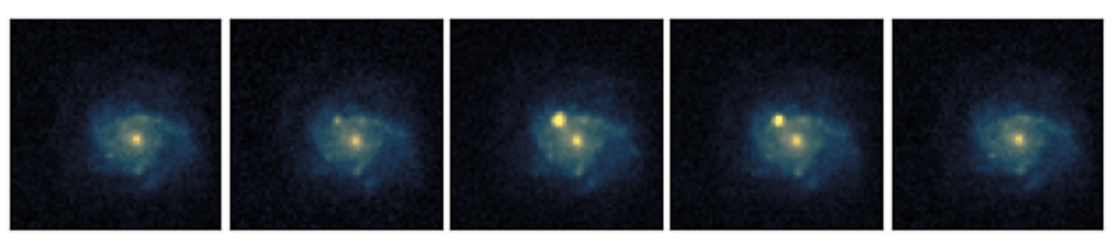
\includegraphics[width=1.0\textwidth]{MainLayout/Third_chapter/figures/ztf_sn_picture.png}
    \caption{Type Ia supernova detected by ZTF. Photos taken accross 2 months (from left to right 20th of Jan 2020, 25th of Jan 2020, 7th of Feb 2020, 20th of Feb 2020, 20th of March 2020). Credits: Mikaël Rigault.}
    \label{fig:ztf_sn_picture}
\end{figure}

\begin{figure}[ht]
    \centering
    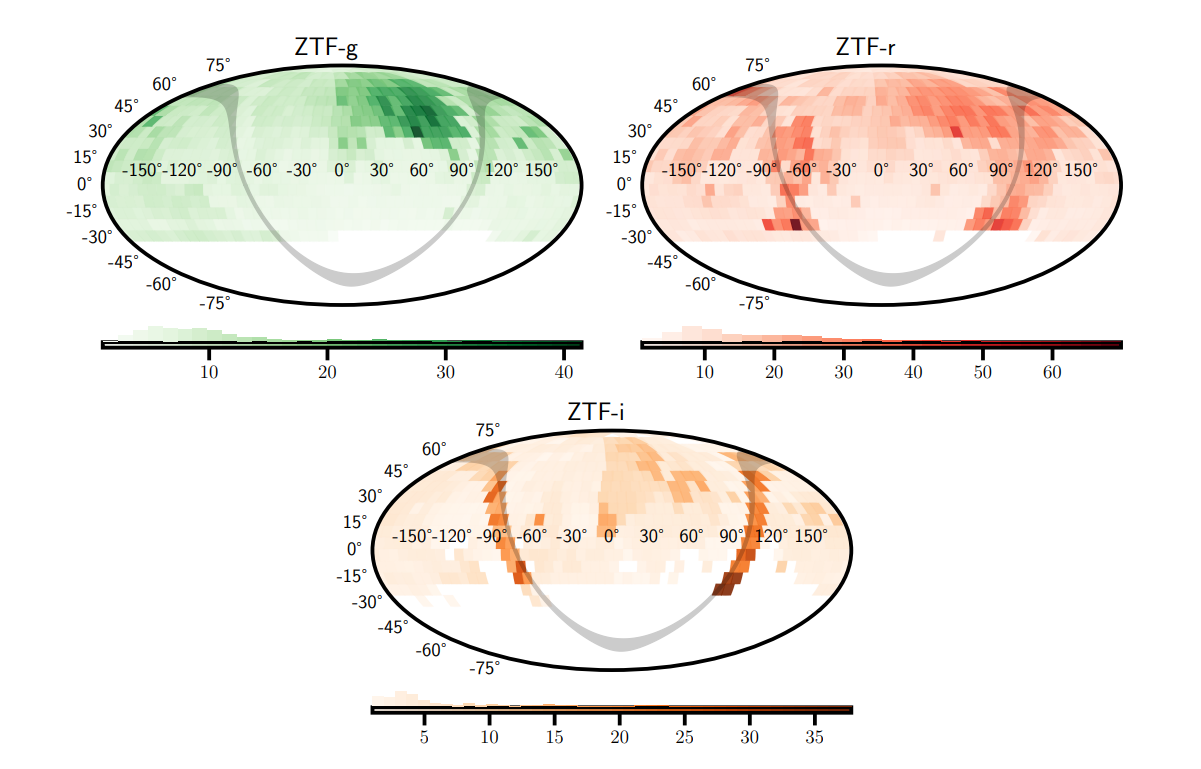
\includegraphics[width=0.8\textwidth]{MainLayout/Third_chapter/figures/ztf_cadence.png}
    \caption{ZTF cadence on the sky. Average number of visits per month for each field of ZTF in each band $g$, $r$ and $i$. Taken from \cite{Carres_2023}}
    \label{fig:ztf_cadence}
\end{figure}

\begin{figure}[ht]
    \centering
    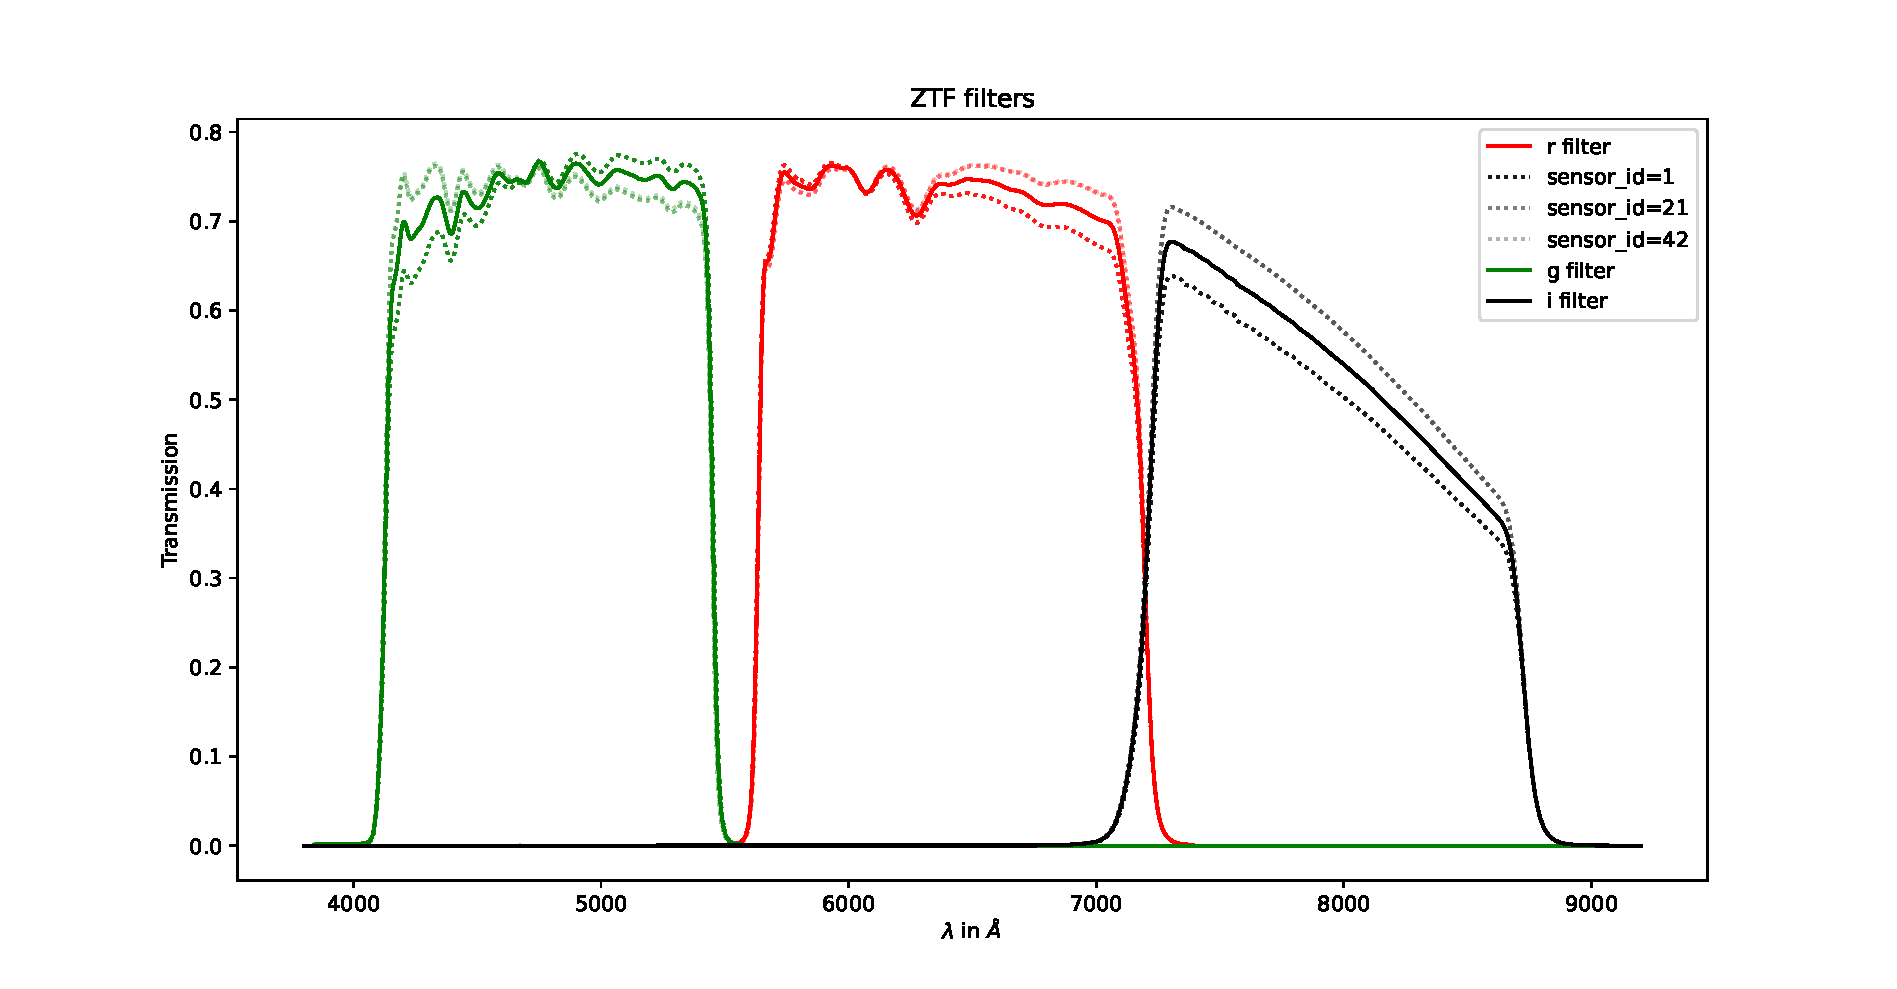
\includegraphics[width=1.0\textwidth]{MainLayout/Third_chapter/figures/ztf_filters.pdf}
    \caption{ZTF filters. Dotted lines represent transmissions for different sensors. Solid lines represent the average transmissions over all sensors.}
    \label{fig:ztf_cadence}
\end{figure}

\subsubsection{Spectroscopic follow up}

ZTF is accompagnied by a spectrograph named the Spectral Energy Distribution Machine (SEDM) located in the same observatory on the P60 telescope. The purpose of the object to 
conduct a follow up on the photometry in order to properly classify the transients obsereved. It's limit magnitude is 20.5mag. This follow up played an important role in acquiring the 
60\% spectra for the ZTF Bright Transient Survey (BTS) for which the magnitude limit was 18.5mag, a limited fraction of the ZTF total survey. \\


\subsubsection{ZTF DR2}

We present in this subsection the type Ia supernova data release of ZTF named DR2. This encompasses data taken from March 2018 and December 2020. The sample contains 3628 
spectroscopically identified supernovae up to a redshift of $z \approx 0.2$. Figure \ref{fig:ztf_lcs} shows examples of the sampling of the supernova obsereved by ZTF in DR2. We must note that not all supernova data is 
"good" enough to be used for a cosmological analysis. For such an analysis, quality cuts on sampling around the maximum emission of light, the color and the stretch must be applied. 
The details on the cosmology quality cuts can be found in \cite{Rigault_2020} and we remind them later in Chapter 4. After the cuts, 
the sample maintains 2667 supernovae that pass. A subset of the sample named the "volume-limited" sample contains all supernovae up to a redshift of $z=0.06$ represents a complete 
sample of supernovae i.e. the sample is not influenced by any selection effects due to the magnitude limits of the telescope. This subset contains 994 supernovae. \\

\begin{figure}[ht]
    \centering
    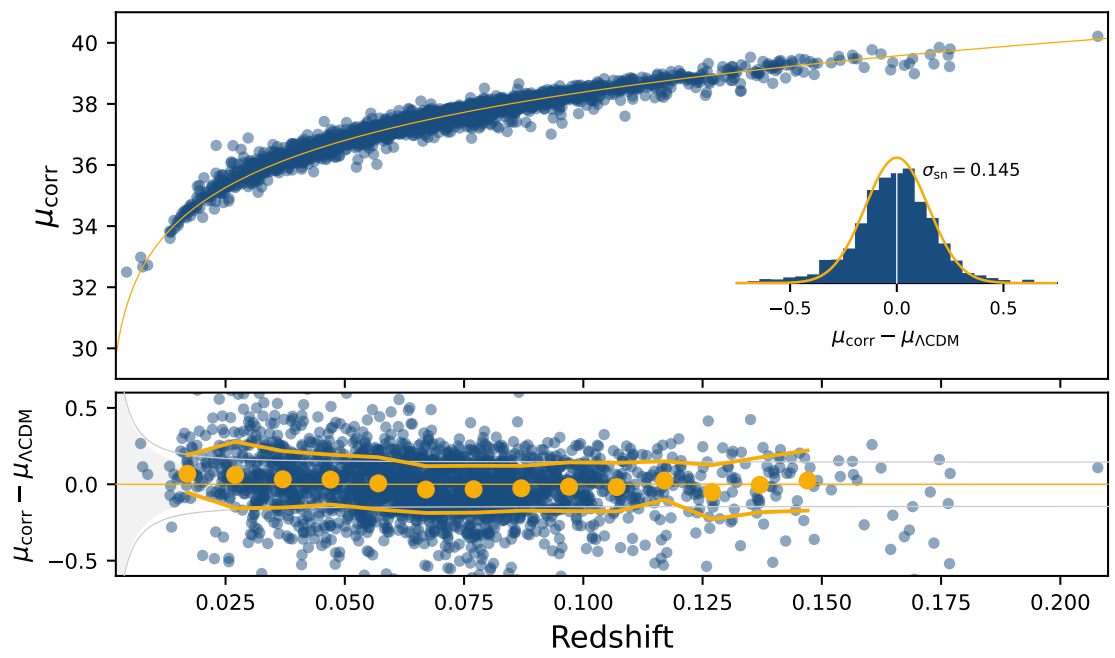
\includegraphics[width=0.8\textwidth]{MainLayout/Third_chapter/figures/ztf_dr2_hubble.png}
    \caption{Hubble diagram created with standardized ZTF DR2 type Ia supernovae compared to fiducial $\Lambda$CDM cosmology anchore on Planck results. Taken from \cite{Rigault_2020}.}
    \label{fig:ztf_dr2_hubble}
\end{figure}

\begin{figure}[ht]
    \centering
    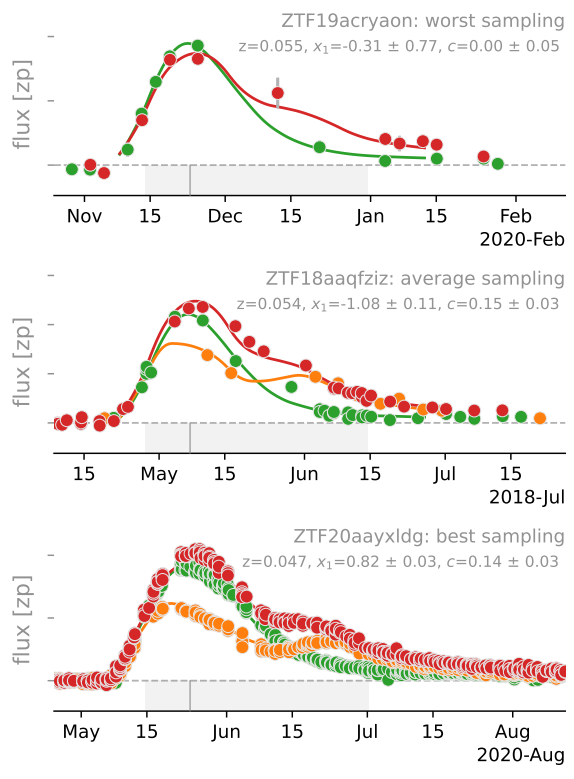
\includegraphics[width=0.5\textwidth]{MainLayout/Third_chapter/figures/ztf_sn_dr2.png}
    \caption{Three supernova Ia lightcurves examples highlighting the worst (top), average (middle) and best (bottom) sampling in DR2. The colors indicate the band they were measured in and the solid lines are the best SALT2 fits. Taken from \cite{Rigault_2020}}
    \label{fig:ztf_lcs}
\end{figure}


\subsection{SNLS survey} \label{sec:snls}

The second dataset is the SuperNova Legacy Survey (SNLS)  (Astier et al., 2006), a type Ia supernova survey conducted with the MegaCam (Boulade et al., 2003) observing system. 
The camera is mounted on the Canada-France-Hawaii 3.6m telescope (CFHT) located on top of the Maunakea volcano, Hawaii.
The focal plane of the MegaCam camera is made up of 40 CCDs (model e2v CCD42-90) each having 
2048 $\times$ 4612 pixels. The CFHT is constructed with two mirrors, the primary mirror has a parabolic shape and is made from a glass-ceramic
material which makes it immune to thermal distortion. The camera is placed in the focal plane of the primary mirror. In addition, a Wide Field
Corrector (WFC) is placed in front of the camera to guarantee a large field of view. \\ 

In order to classify observed supernovae and acquire their redshifts, 
a spectroscopic follow-up is implemented. These additional
observations mostly rely on the European Southern Observatory Very Large Telescope (ESOVLT), 
the Gemini-North and South and the Keck-I and II instruments (Balland et al., 2009;
Astier et al., 2006). As the photometric survey observes more type Ia candidates than what
can be spectroscopically observed afterwards, a target selection process must be implemented. 
In practice, a first light-curves fit is performed in real time which allows to eliminate most of the type II contamination in the survey
For the remaining targets, a limit of mi = 24.5mag (i-band magnitude) has been established, over which a supernova is less
likely to be spectroscopically observed.
The MegaCam camera footprint is a 0.96 × 0.94 = 0.90deg2
rectangle. As a consequence, the chosen observation strategy for SNLS is no longer a wide scan of a large fraction of the sky as for ZTF 
but rather consists is observing deeply (up to z  1) in four
dedicated fields equally distributed in right ascension (see figure 3.10 and table 3.1)
The luminosity of transients is collected through 5 photometric filters, g, r, i, i21
and z,
spanning the visible and near-infrared wavelength ranges. Figure 3.11 presents the transmission of the SNLS filters as a function of wavelength. 
As for ZTF earlier, we highlight the
fact that the transmissions are sensor-dependent by displaying the average transmission
over the focal plane and a transmission curve for four different sensors.
In this thesis, the analysed SNLS data consists in the five years survey (SNLS 5y), which
started in the second half of 2003 and ended in 2009. The dataset comprises SNLS 3y data
as well as data from the 4th and 5th years which will be published in Betoule et al. in prep.
Figure 3.12 presents the number of exposures per day as a function of time for the entire
SNLS survey. \\


\subsection{HSC survey} \label{sec:hsc}


The Hyper Suprime-Cam Subaru Strategic Program (Aihara et al., 2022), also denoted HSCSSP, is an astronomical 
observation program which allocated some telescope time to the 
observation of type Ia supernovae at the end of the 2010’s. Its primary system is the Hyper
Suprime Cam, a camera mounted on the Subaru 8.2m telescope. As for the CFHT, the
Subaru telescope is located on top of the Maunakea volcano, Hawaii (see figure 3.13).
The focal plane of the Hyper Suprime-Cam camera includes 116 Hamamatsu CCDs 
each totalizing 2048 × 4096 = 8.4Mpx (Hyper Suprime Cam documentation). The Subaru
telescope also follows a Prime Focus architecture. Figure 3.14 presents a side view of the
Hyper Suprime Cam mounted on the Subaru telescope.
The redshifts of the HSC supernovae are determined by measuring the redshift of their
host galaxies. These redshifts were mainly collected by the AAT/AAOmega and DESI
instruments, completed by observations from the Subaru/FOCAS and VLT instruments
(Suzuki et al. in prep). As of today, around 500 redshifts have been measured and observations are still going on, in particular in the XMM field (see figure 3.15).
The HSC-SSP collaboration also developed four methods to determine the redshifts directly from photometry. The Direct Empirical Photometric method (DEmP) and the TPZ
method both rely on machine learning to infer redshifts. The first approach consists in
fitting a polynomial function modeling the redshift as a function of magnitude (Hsieh and
Yee, 2014) while the second one uses random forest algorithms (Carrasco Kind and Brunner,
2013). For complementary measurements, the LePhare and MIZUKI methods both relies on
template fitting with priors. While the LePhare approach uses redshift distributions priors
from the 30-band photometric redshifts of the COSMOS survey (Ilbert et al., 2009; Coupon
et al., 2015), the MIZUKI approach uses Bayesian priors (Tanaka, 2015). 
The Hyper Suprime-Cam camera footprint is a 1.8deg2 disc which is about twice the
size of the MegaCam footprint. Although the main focus of the HSC-SSP is to build a galaxy
catalog for weak lensing analysis, the observation cadence of its deep fields were adapted
for supernovae observation. Because the main goal of the HSC supernova survey is to
observe faint transients at high redshift (up to z  1.6), the chosen observation strategy
is also similar to SNLS. In fact, the supernovae observation is restricted to four dedicated
deep fields (XMM-LSS, E-COSMOS, ELAIS-N1, DEEP2-F3) and two ultra-deep fields (SXDS
and COSMOS), partially overlapping the SNLS D1 and D2 fields respectively. Figure 3.15
presents a summary of the HSC deep and ultra-deep fields locations. 
The luminosity of transients is collected through 7 photometric filters, g, r, r22
, i, i2, z
and y, spanning the visible and near-infrared wavelength ranges. Figure 3.16 presents the
transmission of the HSC filters as a function of wavelength. Although the transmissions are
sensor-dependent as for the ZTF and SNLS filters, we only display the average transmission
curves over the focal plane for clarity.

In this thesis, the analysed HSC data consists in the HSC supernova survey, which
started with a first observation season in 2017 and ended with a second observation season
in 2020. Figure 3.17 presents the number of exposures per day as a function of time for the
entire HSC survey

\subsection{Pipeline overview}
\subsection{Cosmological analyses with LEMAITRE}
\subsection{Uncertainties in SN measurements?}
